% !TeX encoding = UTF-8
\chapter{Task 4: Real-Time Classification}\label{chap:task4_realtime}

\section{Setup}\label{sec:realtime-setup}

For the real-time part, we use the binary default Decision Tree (\texttt{binary\_dt\_default}). It has the best DDoS F1 and the fewest errors on the test split (7 false positives among 28,521 benign flows and 25 false negatives among 38,404 DDoS flows). The detector loads the saved pipeline unchanged, so training and serving use exactly the same scaling, selection and classifier. Figure~\ref{fig:arch} shows the data flow. The input is the flow CSV of our own capture (Chapter~\ref{chap:task1_flows}): 569 flows produced by CICFlowMeter V4, whereas the training data comes from an older version. The detector streams the flows one by one in timestamp order, maps the V4 column names to the training names (all 77 features map), drops the \texttt{Protocol = 0} rows, replaces infinite and NaN values by 0 and classifies each flow (Listing~\ref{lst:detector}). The flow CSV is a command-line argument, so the detector can be pointed at any other V4 flow file.

\begin{figure}[ht]
	\centering
	\resizebox{\linewidth}{!}{%
	\begin{tikzpicture}[node distance=5mm, every node/.style={font=\footnotesize},
		box/.style={draw, rounded corners=2pt, align=center, minimum height=1.6cm, minimum width=2.3cm, text width=2.2cm, fill=gray!10},
		>={Stealth[length=2mm]}]
		\node[box] (a) {Capture\\\texttt{.pcapng}};
		\node[box, right=of a] (b) {CICFlowMeter\\(offline)};
		\node[box, right=of b] (c) {Flow CSV\\(V4 columns)};
		\node[box, right=of c] (d) {Column\\mapping\\V4 $\to$ training};
		\node[box, right=of d] (e) {Clean:\\drop\\\mbox{Protocol 0},\\inf/NaN $\to$ 0};
		\node[box, right=of e] (f) {Pipeline\\(scale, select,\\tree)};
		\node[box, right=of f] (g) {Verdict\\per flow};
		\foreach \x/\y in {a/b,b/c,c/d,d/e,e/f,f/g} \draw[->] (\x) -- (\y);
	\end{tikzpicture}}
	\caption{Real-time architecture. Flows are streamed row by row in timestamp order.}
	\label{fig:arch}
\end{figure}

\lstinputlisting[style=py,float=htbp,linerange={36-42,44-46,48,50-52,61-65},caption={Excerpt of \texttt{Detector.process()} in \texttt{src/ddosids/realtime/detector.py}: column mapping, Protocol-0 drop, feature check, inf/NaN replacement and prediction (some lines omitted)},label={lst:detector}]{../src/ddosids/realtime/detector.py}

\section{Correctness: Parity Test}\label{sec:parity}

To prove that the real-time path does not change the model's behavior, an end-to-end test converts the 66,925-flow test split to the V4 column names and streams it through the detector. The streamed predictions are identical, row for row, to those of the offline pipeline, both for batches of 1,000 flows and, on the first 500 flows, for batches of one flow. The DDoS F1 recomputed from the streamed predictions equals the offline value of Table~\ref{tab:t4binary}. Figure~\ref{fig:tests} shows the test evidence: 24 fast tests pass (3 slow end-to-end tests deselected), and the 3 end-to-end tests (Task 3 numbers, Task 4 regression guards and this parity test) pass as well.

\begin{figure}[ht]
	\centering
	\begin{subfigure}[t]{0.45\linewidth}
		\centering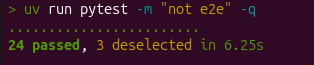
\includegraphics[width=\linewidth]{SS36.png}
		\caption{Fast tests: 24 passed, 3 deselected.}
	\end{subfigure}\hfill
	\begin{subfigure}[t]{0.45\linewidth}
		\centering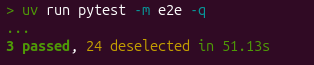
\includegraphics[width=\linewidth]{SS37.png}
		\caption{End-to-end tests: 3 passed, 24 deselected.}
	\end{subfigure}
	\caption{Test evidence for Tasks 3 and 4.}
	\label{fig:tests}
\end{figure}

\section{Results on Our Capture}\label{sec:realtime-results}

Of 569 flows, 22 were dropped (protocol 0) and 547 were classified, all of them as BENIGN: the detector raised 0 DDoS alerts (Table~\ref{tab:t5rt}, Figure~\ref{fig:ss38}). No infinite or NaN cells had to be replaced. Our traffic is benign by construction, so every flow is correctly classified and there is no false positive.

\begin{table}[ht]
	\centering\small
	% AUTO-GENERATED by scripts/make_report_tables.py from outputs/realtime/run_log.txt, outputs/realtime/predictions.csv -- do not edit
\begin{tabular}{lr}
\toprule
Quantity & Value \\
\midrule
Flows read & 569 \\
Protocol-0 flows dropped & 22 \\
inf/NaN cells replaced & 0 \\
Flows classified & 547 \\
Classified BENIGN & 547 \\
DDoS alerts & 0 \\
Alert rate & 0.00\,\% \\
Latency per flow, mean (ms) & 13.537 \\
Latency per flow, median (ms) & 12.840 \\
\bottomrule
\end{tabular}

	\caption{Real-time run on \texttt{task2\_lab2.pcap\_Flow.csv}.}
	\label{tab:t5rt}
\end{table}

\ssfig[0.6\linewidth]{SS38}{Summary of the real-time detector: 569 flows read, 22 Protocol-0 rows dropped, 547 classified, 0 DDoS alerts, mean latency 13.537\,ms per flow.}{fig:ss38}

\section{Latency and Scope}\label{sec:latency}

Classifying one flow at a time takes 13.537\,ms on average (median 12.840\,ms) in our recorded run. This is per-call pandas and scikit-learn overhead: batched, the same model needs 0.695\,ms per 1,000 flows (Table~\ref{tab:t4binary}). In practice, the detection delay is dominated by CICFlowMeter, which emits a flow only when it ends (FIN or RST) or times out (5\,s activity, 120\,s flow timeout). ``Real time'' here means streaming the flows of a recorded capture through the detector one by one; we do not capture packets live.

\paragraph{Limitations of this check.} Our capture contains only benign traffic, so we can measure the false-positive behavior on our network but not the detection rate: whether the model would flag a real DDoS attack in our flows remains untested. In addition, there is domain shift. The training data was produced by an older CICFlowMeter version on the 2017 testbed, whereas our flows come from CICFlowMeter V4 on a different network with a different application mix (for example QUIC and Steam traffic). A model that relies on testbed-specific shortcut features, such as the destination port, may behave differently on other traffic, in either direction.

\FloatBarrier
